%% Basierend auf einer Vorlage des SDQ
%% Siehe https://sdqweb.ipd.kit.edu/wiki/Dokumentvorlagen


%% complexity classes
\renewcommand{\P}{\ensuremath{\mathcal{P}}\xspace}
\newcommand{\NP}{\ensuremath{\mathcal{NP}}\xspace}
\newcommand{\ParaNP}{\ensuremath{para-\mathcal{NP}}\xspace}
\newcommand{\XP}{\ensuremath{\mathcal{XP}}\xspace}
\newcommand{\FPT}{\ensuremath{\mathcal{FPT}}\xspace}
\newcommand{\N}{\ensuremath{\mathbb{N}}\xspace}

\newcommand{\BigO}[1]{\ensuremath{\operatorname{\mathcal{O}}\bigl(#1\bigr)}\xspace}
\newcommand{\blue}[1]{\textcolor{kit-blue100}{#1}\xspace}
\newcommand{\red}[1]{\textcolor{kit-red100}{#1}\xspace}


%% Beispiel-Präsentation
\documentclass[navbaroff]{sdqbeamer} 
%\usepackage{complexity}
\usepackage{tikz}
\usepackage{xspace}
\usepackage{wasysym}

\usepackage[most]{tcolorbox}

\renewcommand{\note}[1]{
    \begin{minipage}{0.3\textwidth}
        \begin{blueblock}{}
            #1
        \end{blueblock}
    \end{minipage}
}

\newtcolorbox{Qbox}{
enhanced,
sharp corners,
rounded corners=northeast,
rounded corners=southwest,
sidebyside,
colback=kit-red15,
colframe=kit-red15,
righthand width=25pt,
height from=38pt to \pdfpageheight,
valign=center,
overlay={\node[xshift=-30pt] at (frame.east) 
    {
        \includegraphics[height=25pt]{QM.png}
    };
  }
}

\newcommand\questionbox[1]{%
  \begin{Qbox}
        #1
  \end{Qbox}
}

\newtcolorbox{Abox}{
enhanced,
sharp corners, 
rounded corners=northeast,
rounded corners=southwest,
sidebyside,
colback=kit-green15,
colframe=kit-green15,
righthand width=25pt,
height from=38pt to \pdfpageheight,
valign=center,
overlay={\node[xshift=-30pt] at (frame.east) 
    {
        \includegraphics[height=30pt]{AW.png}
    };
  }
}

\newcommand\answerbox[1]{%
  \begin{Abox}
        #1
  \end{Abox}
}

%% Titelbild
\titleimage{banner_2020_kit}

%% Gruppenlogo
\grouplogo{} 

%% Gruppenname und Breite (Standard: 50 mm)
\groupname{Proseminar Algorithmen für NP-schwere Probleme}
%\groupnamewidth{50mm}

% Beginn der Präsentation

\title[Parametrisierte Algorithmen II]{Parametrisierte Algorithmen II}
\subtitle{Hauptvortrag} 
\author[Oliver Enes]{Oliver Enes}

\date[05.06.2023]{05. Juni 2023}

% Literatur 
 
\usepackage[citestyle=authoryear,bibstyle=numeric,hyperref,backend=biber]{biblatex}

\addbibresource{presentation.bib}
\bibhang1em

\begin{document}
 
%Titelseite
\KITtitleframe

\begin{frame}[t]{Wofür parametrisierte Algorithmen?}
    
    \visible<2->{
        \begin{itemize}
            \item Viele Probleme sind \NP-schwer
        \end{itemize}
    }

    \visible<3->{
        \vspace{20pt}
        \questionbox{
            \centering
            \textbf{Ist damit jede Instzanz eines \NP-schweren Problems nicht effizient lösbar?}
        }
    }
    
    \visible<4->{
        \answerbox{
            \centering
            \textbf{
                In der Praxis sind viele Instanzen \NP-schwerer Probleme effizient lösbar, weil die Instanzen \blue{gutartig} sind!
            }
        }
    }

    \visible<5->{
        \vspace{20pt}
        \centering
        \textbf{Parametrisierte Algorithmen formalisieren Gutartigkeit}
    }

\end{frame}

\begin{frame}{Parametrisiertes Problem}

    \begin{blueblock}{Parametrisiertes Problem}
        Ein \blue{parametrisiertes Problem} ist eine Sprache $ L \subseteq \Sigma^* \times \blue{\N} $ wobei $\Sigma$ ein endliches Alphabet ist.
        \\
        Die zweite Komponente heißt \blue{Parameter}.
    \end{blueblock}

    
    \visible<2-3>{
        \large{\textbf{Beispiele:}}
        \vspace{10pt}
        \begin{center}
            \begin{tabular}{ |c|c| } 
             \hline
             Problem & Parameter \\
             \hline
             \textsc{k-Vertex-Cover} & k \\
             \hline
             \textsc{Subset Sum} & Summe aller Elemente \\
             \hline
             \textsc{3Color} & größte Cliquengröße \\
             \hline
             \textsc{k-Vertex-cover} &  $min_{v \in V(G)}{deg(v)}$ \\
             \hline
            \end{tabular}
        \end{center}
    }

    \visible<3>{
        \vspace{5pt}
        \large{\textbf{Anmerkungen:}}
        \begin{itemize}
            \item Parameter i.A. nicht eindeutig
        \end{itemize}
    }
\end{frame}

\begin{frame}{Parametrisierte Komplexität}
    \visible<2->{
        \begin{blueblock}{Problemklasse \FPT}
            Ein parametrisiertes \textbf{Entscheidungsproblem} heißt \blue{FPT (Fixed-Parameter-Tractable)},
            wenn ein Algorithmus existiert, der alle Probleminstanzen (x, k) in \BigO{\blue{f(k)} \cdot \textcolor{kit-red100}{|x|^c}} löst, wobei $ c \in \N $ und $f$ beliebige berechenbare Funktion ist.
            
            \vspace{10pt}
            Die Menge aller solcher Probleme bildet die Problemklasse \blue{\FPT}.
        \end{blueblock}  
    }
    
    \visible<3-4>{
        \vspace{5pt}
        \large{Beispiele:}
        \begin{itemize}
            \item \BigO{\blue{(43k^2+k)} \cdot \textcolor{red}{|x|^2}}
            \item \BigO{\blue{2^k} \cdot \textcolor{red}{(|x|^3+42|x|)}}
            \item \BigO{\textcolor{kit-red100}{|x|^{123}+12}}
            \item \BigO{\blue{\varphi(k, k - 5, k - \sqrt{k})} \cdot \textcolor{kit-red100}{\log(|x + 1|)}} wobei $\varphi$ die Ackermann-Funktion ist.
        \end{itemize}
    }

    \visible<4>{
        \textbf{Beobachtung:} Für festes $k$ ist die Laufzeit polynomiell in der Eingabegröße.
    }

\end{frame}


\begin{frame}[t]{Ein \NP-schweres Problem: \textsc{Vertex-Cover}}
    \begin{redblock}{Problem \textsc{k-Vertex-Cover}}
            \textbf{Eingabe}: Graph $G = (V, E)$, $k \in \mathbb{N}$
            \\
            \textbf{Parameter}: Lösungsgröße $k$
            \\
            \textbf{Frage}: Existiert Menge $M \subseteq V$, sodass $|M| \leq k$ und jede Kante zu mindestesns einem Knoten in $M$ adjazent ist?
    \end{redblock}%
    \begin{overlayarea}{\textwidth}{\textheight}
        \onslide*<2-3>{%
            \centering
            \begin{overprint}
                \begin{figure}
                    \includegraphics<2>[width=200pt]{images/vertex-cover-1.eps}%
                    \includegraphics<3>[width=200pt]{images/vertex-cover-1b.eps}%
                \end{figure}
                (\textbf{hier:} $k = 4$)
            \end{overprint}
        }%
        \onslide*<4->{%
            \begin{columns}[T]
                \begin{column}{0.5\linewidth}
                    \begin{center}
                        \begin{greenblock}{Satz}
                            \textsc{Vertex-Cover} ist \NP-vollständig.
                        \end{greenblock}
                        \visible<5->{
                            \vspace{25pt}
                            \centering
                                \textbf{
                                    \textcolor{kit-blue100}{Wie lässt sich die Instanz vereinfachen?}
                                }
                        }
                    \end{center}
                \end{column}
                \begin{column}{0.45\linewidth}
                    \begin{figure}
                        \includegraphics[width=175pt]{images/vertex-cover-1.eps}
                    \end{figure}
                    \centering
                    (\textbf{hier:} $k = 4$)
                \end{column}
            \end{columns}
        }%
    \end{overlayarea}
\end{frame}

\begin{frame}{}
    \vspace{25pt}
    \begin{overlayarea}{1\textwidth}{1\textheight}
        \centering
        \begin{figure}
            \onslide*<1-2>{%
            \includegraphics[width=200pt]{images/vertex-cover-1.eps}%
            }%
            \onslide*<3->{%
                \includegraphics[width=200pt]{images/vertex-cover-2.eps}%
            }%
        \end{figure}
        
        (\textbf{hier:} $k = 4$)
        \vspace{5pt}
        \onslide*<1-2>{%
        \questionbox{
            \centering
            Wie lässt sich die Instanz vereinfachen?
        }
        }%
        \onslide*<3>{%
            \answerbox{
                \centering
                Isolierte Knoten können vernachlässigt werden.
            }
        }%
        \onslide*<4->{%
            \begin{lightgreenblock}{1. Reduktionsregel}
                Ist $(G, k)$ eine \textsc{k-Vertex-Cover} Instanz mit Parameter $k$ und $U$ die Menge der isolierten Knoten in G, \\ so ist $(G-U, k)$ eine äquivalente Instanz.
            \end{lightgreenblock}
        }%
        \onslide*<5->{%
            \textbf{Beweis:} Da isolierte Knoten mit keiner Kante verbunden sind,
            tragen sie nicht zur Kantenabdeckung bei.
        }%
    \end{overlayarea}%
    \visible<2->{%
        \tikz[overlay, remember picture] \node[xshift=-28mm, yshift=-14mm] at (current page.north east) {
            \note{
                Instanzen sind \blue{äquivalent}, wenn die vereinfachte Instanz Ja-Instanz ist, gdw. die ursprüngliche Instanz Ja-Instanz ist.
            }
        };
    }%
\end{frame}

\begin{frame}{}
    \vspace{25pt}
    \begin{overlayarea}{1\textwidth}{1\textheight}
        \centering
        \begin{figure}
            \onslide*<1>{%
                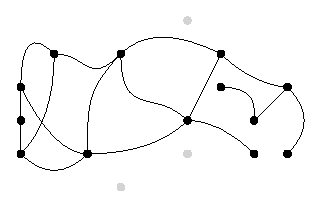
\includegraphics[width=200pt]{images/vertex-cover-3.eps}%
            }%
            \onslide*<2->{%
                \includegraphics[width=200pt]{images/vertex-cover-4.eps}%
            }%
        \end{figure}
        (\textbf{hier:} $k = 4$)
        \vspace{5pt}
        \onslide*<1>{%
            \questionbox{
                \centering
                Wie lässt sich die Instanz vereinfachen?
            }
        }%
        \onslide*<2>{%
            \answerbox{
                \centering
                Wenn ein Knoten Grad mindestesns $k+1$ hat, ist er im Vertex Cover enthalten.    
            }
        }%
        \onslide*<3->{%
            \begin{lightgreenblock}{2. Reduktionsregel}
                Ist $(G, k)$ eine \textsc{k-Vertex-Cover} Instanz mit Parameter $k$ und $v \in V(G)$ Knoten mit $deg(v) \geq k+1$, so ist $(G-v, k-1)$ eine äquivalente Instanz.
            \end{lightgreenblock}
        }%
        \onslide*<4>{%
            \raggedright
            \textbf{Beweis:}
            \\
            \enquote{$\Rightarrow$}:
            \\
            Sei G eine Ja-Instanz mit Vertex Cover $M$.
            \\
            G-v hat das Vertex Cover $M' = M\setminus{\{v\}}$. $|M'| = |M| - |\{v\}| \leq k - |\{v\}| = k - 1$.
        }%
        \onslide*<5->{
            \raggedright
            \textbf{Beweis:}
            \\
            \enquote{$\Leftarrow$}:
            \\
            Sei $G-v$ eine Ja-Instanz mit Vertex Cover $M'$.
            Wird $v$ hinzugefügt, deckt $v$ alle neuen Kanten ab.
            \\
            G hat Vertex Cover $M = M' \cup \{v\}$.
    }
    \end{overlayarea}%
    \visible<1->{
        \tikz[overlay, remember picture] \node[xshift=-28mm, yshift=-14mm] at (current page.north east) {
            \note{
                Instanzen sind \blue{äquivalent}, wenn die vereinfachte Instanz Ja-Instanz ist, gdw. die ursprüngliche Instanz Ja-Instanz ist.
            }
        };
    }%
\end{frame}

\begin{frame}{}
    \vspace{25pt}
    \begin{overlayarea}{1\textwidth}{1\textheight}
        \centering
        \begin{figure}
            \onslide*<1>{%
            \includegraphics[width=200pt]{images/vertex-cover-5.eps}%
            }%
            \onslide*<2>{%
                \includegraphics[width=200pt]{images/vertex-cover-6.eps}%
                \tikz[overlay, remember picture] \node[xshift=-75mm, yshift=-37mm] at (current page.north east) {%
                    \large%
                    \textcolor{kit-red100}{\textbf{1. Regel}}%
                };%
            }%
            \onslide*<3>{%
                \includegraphics[width=200pt]{images/vertex-cover-7.eps}%
            }%
            \onslide*<4>{%
                \includegraphics[width=200pt]{images/vertex-cover-8.eps}%
                \tikz[overlay, remember picture] \node[xshift=-125mm, yshift=-40mm] at (current page.north east) {%
                    \large%
                    \textcolor{kit-red100}{\textbf{2. Regel}}%
                };%
            }%
            \onslide*<5->{%
                \includegraphics[width=200pt]{images/vertex-cover-9.eps}%
            }%
        \end{figure}
        (\textbf{hier:} $k = 4$)
        \vspace{5pt}
        \onslide*<1-5>{%
            \questionbox{
                \centering
                Wie lässt sich die Instanz vereinfachen?
            }
        }%
        \onslide*<6>{%
            \answerbox{
                \centering
                Hat der Graph nach erschöpfender Anwendung von Regel 2 mehr als $k^2$ Kanten, ist $(G, k)$ eine Nein-Instanz.
            }
        }%
        \onslide*<7->{%
            \begin{lightgreenblock}{3. Reduktionsregel}
                Ist $(G, k)$ eine \textsc{k-Vertex-Cover} Instanz mit $deg(v) \leq k$ für alle $v \in V(G)$ und $|E(G)| > k^2$, ist $(G, k)$ eine Nein-Instanz.
                Gib in diesem Fall eine triviale Nein-Instanz zurück.
            \end{lightgreenblock}
        }%
        \onslide*<8->{%
            \raggedright
            \textbf{Beweis:}
            \\
            Vertex Cover $M$ von $k$ Knoten kann maximal $\displaystyle\sum_{v \in M}^{}{deg(v)} \leq \sum_{v \in M}^{}{k} = k \cdot k = k^2$ abdecken.
        }%
    \end{overlayarea}%
    \visible<1->{
        \tikz[overlay, remember picture] \node[xshift=-28mm, yshift=-14mm] at (current page.north east) {
            \note{
                Instanzen sind \blue{äquivalent}, wenn die vereinfachte Instanz Ja-Instanz ist, gdw. die ursprüngliche Instanz Ja-Instanz ist.
            }
        };
    }%
\end{frame}

\begin{frame}{Zwischenergebnis}
    \begin{center}
        \includegraphics[width=320pt]{images/reduction-rules.eps}
    \end{center}

    \visible<2>{
        \vspace{5pt}
        \centering
        \textbf{
            Wie sieht der Graph nach erschöpfender Anwendung der Reduktionsregeln aus?
        }
    }
\end{frame}

\begin{frame}[t]{Ein Problemkern für \textsc{Vertex-Cover}}
    \begin{greenblock}{Satz}
        Eine \textsc{k-Vertex-Cover} Instanz (G, k) reduziert sich nach erschöpfender Anwendung\\ der Reduktionsregeln 1 - 3 auf eine Größe in \BigO{k^2}.
    \end{greenblock}
    \visible<2->{
        \raggedright
        \textbf{Beweis:}
        \\
        Sei $\tilde{G}$ der Graph, der aus einer \textsc{k-Vertex-Cover} Instanz $(G, k)$ nach erschöpfender Anwendung der Reduktionsregeln 1-3 entstanden ist.
        \\
        \visible<3->{
            Zu zeigen: $|V(\tilde{G})|, |E(\tilde{G})| \in \BigO{k^2}$
            \\
        }
        \begin{columns}
            \begin{column}{0.57\textwidth}
                \begin{overlayarea}{1\textwidth}{1\textheight}
                    \begin{itemize}
                        \item<4-> Durch Anwendung von 1. besitzt $\tilde{G}$ keine isolierten Knoten.
                        \\
                        (also ist jeder Knoten zu mindestens einer Kante adjazent)
                        \item<5-> Durch Anwendung von 3. existieren max. $k^2$ viele Kanten.
                        
                        \visible<6->{
                            $\Rightarrow$ Damit existieren maximal $2k^2$ viele Knoten.
                        }
                    \end{itemize}
                \end{overlayarea}
            \end{column}
            \begin{column}{0.43\textwidth}
                \raggedright
                \vspace{5pt}
                \begin{overlayarea}{1\textwidth}{1\textheight}
                    \onslide*<7>{
                        \questionbox{\centering Wo haben wir die \\2. Reduktionsregel gebraucht?}
                    }
                
                    \onslide*<8>{
                        \answerbox{\centering Die 3. Regel setzt die 2. voraus, damit jeder Knoten maximal $k$ Kanten hat.}
                    }
                
                    \onslide*<9->{
                        \centering
                        \begin{itemize}
                            \item[] \textbf{Die Problemgröße ist nur noch vom Parameter abhängig!}
                            \item<10->[] \textbf{Alle Reduktionen sind in polynomieller Zeit durchführbar!}
                        \end{itemize}
                    }
                \end{overlayarea}
            \end{column}
        \end{columns}
    }

\end{frame}

\begin{frame}[t]{Problemkerne \& Problemkernreduktion}
    \visible<2->{
        \begin{itemize}
            \item \textbf{Ziel:} gerade gesehene Konzepte verallgemeinern und formalisieren
        \end{itemize}
    }

    \visible<3->{
        \begin{blueblock}{Problemkern \& Problemkernreduktion}
            Sei $ P \subseteq \Sigma^* \times \N $ ein parametrisiertes Problem.
            \\
            Es bezeichne $|I|$ die (Eingabe-)Größe einer Probleminstanz $I := (x, k) \in \Sigma^* \times \N$.
            \\
            Eine \blue{Problemkernreduktion} $ \blue{\Phi: \Sigma^* \times \N \rightarrow \Sigma^* \times \N }$ ist eine Funktion sodass:
            \begin{itemize}
                \item $I \in P \iff I' := \blue{\Phi(I)} \in P $
                \item $|I'| \leq f(k)$ für eine beliebige Funktion $f: \N \rightarrow \N$
                \item \blue{$\Phi$} ist polynomiell in $|x| + k$ berechenbar
            \end{itemize}
            \vspace{10pt}
            $ I' $ heißt \blue{Problemkern} von $I$.
        \end{blueblock}

        \only<4->{
            \textbf{Anmerkungen:}
            \begin{itemize}
                \item Insbesondere ist die Größe des Problemkerns nur von $k$ abhängig.
            \end{itemize}
        }
    }
\end{frame}

\begin{frame}[t]{Problemkerne \& \FPT}

    \visible<3-9>{
        \tikz[overlay, remember picture] \node[xshift=-30mm, yshift=-48mm] at (current page.north east) {
            \note{
                \blue{FPT},
                wenn Algorithmus existiert, der alle Probleminstanzen (x, k) in \BigO{\blue{f(k)} \cdot \textcolor{kit-red100}{|x|^c}} löst.
            }
        };
    }
    \visible<10->{
        \tikz[overlay, remember picture] \node[xshift=-30mm, yshift=-53mm] at (current page.north east) {
            \note{
                \begin{minipage}{120pt}
                    \raggedright
                    \small
                    \setlength\leftmargini{15pt}
                    \begin{itemize}
                        \item $I \in P \iff I' := \Phi(I) \in P $
                        \item $|I'| \leq f(k)$ für eine beliebige\\ Funktion $f: \N \rightarrow \N$
                        \item $\Phi$ ist polynomiell in $|x| + k$\\berechenbar.
                    \end{itemize}
                \end{minipage}
            }
        };
    }
    \only<1-2>{
        \begin{blueblock}{}
            \textbf{Erinnerung}
            \\
            Ein parametrisiertes \textbf{Entscheidungsproblem} heißt \blue{FPT (Fixed-Parameter-Tractable)},
            wenn ein Algorithmus existiert, der alle Probleminstanzen (x, k) in \BigO{\blue{f(k)} \cdot \textcolor{kit-red100}{|x|^c}} löst.
        \end{blueblock}
    }
    \only<2->{
        \begin{greenblock}{\FPT \& Problemkerne}
            Ein Problem besitzt genau dann einen Problemkern wenn es in \FPT ist.
        \end{greenblock}
    }
    \visible<3->{
        \textbf{Beweis:}
        \\
    }
    \begin{overlayarea}{1\textwidth}{1\textheight}
        \onslide*<4-9>{
            $\Rightarrow$:
            \begin{itemize}
                \item<5-> Sei $(x, k)$ Probleminstanz eines parametrisierten Problems P\\ mit Problemkernreduktion $\Phi$.
                \item<6-> Es ex. Algorithmus $\mathcal{A}$ der in polynomieller Zeit eine Lösung für P überprüfen kann.
                \item<7-> Erzeuge Problemkern $(x', k') := \Phi(x, k) $.
                \item<8-> Löse $(x', k')$ mittels $\mathcal{A}$, indem alle mögichen Lösungen systematisch probiert werden.
                \item<9-> Damit ist die Laufzeit in \BigO{\qquad \underbrace{p(|x| + k)}_{\textrm{Laufzeit von $\Phi$}} \qquad + \underbrace{\textcolor{kit-blue100}{f(k)}}_{\textrm{Alle Löungen probieren}} \cdot \underbrace{\textcolor{kit-red100}{|x|^c}}_{\textrm{Lösung überprüfen}}} $ = $ \BigO{\textcolor{kit-blue100}{f(k)} \cdot \textcolor{kit-red100}{|x|^c}},\\ wobei $f$ die Laufzeit für das Auflisten aller Lösungsvorschläge und $p$ beliebiges Polynom ist.
            \end{itemize}
        }
        \onslide*<10-19>{
        $\Leftarrow$:
            \\
            \visible<11->{
                Es sei $(x, k)$ eine Instanz eines \FPT-Problems P.
            }
            \\
            \vspace{8pt}
            \only<12-17>{
                \textbf{Fall 1:} $|x| > f(x)$
                \\
                Konstruiere Problemkernreduktion $\Phi$ wie folgt:
                \begin{itemize}
                    \item<13-> Es exisitiert ein Algoritmus $\mathcal{A}$ der P in \BigO{\textcolor{kit-blue100}{f(k)} \cdot \textcolor{kit-red100}{|x|^c}} löst.
                    \item<14-> Lasse $\mathcal{A}$ die Instanz lösen.
                    \item<15-> Ist $(x, k)$ eine Ja-Instanz, gib eine triviale Ja-Instanz zurück.
                    \item<16-> Andernfalls gib eine triviale Nein-Instanz zurück.
                    \item<17-> Laufzeit in \BigO{\textcolor{kit-red100}{|x|^{c+1}}} und damit polynomiell in $|x| + k$.
                \end{itemize}
                }
                \only<18->{
                    \textbf{Fall 2:} $|x| \leq f(x)$
                    \\
                    \visible<19->{
                        Dann ist bereits $|x| \leq f(k)$. Gib $(x, k)$ zurück.
                    }
                }
        }
        \onslide*<20->{
            \vspace{10pt}
            \includegraphics{images/reduction-proof.eps}
        }
    \end{overlayarea}
\end{frame}

\begin{frame}{Zusammenfassung Problemkerne \& Problemkernreduktion}
    \begin{itemize}
        \item Problemkerne isolieren den Teil einer Probleminstanz indem die Schwierigkeit liegt.
        \item Die Größe eines Problemkerns hängt nur vom Parameter ab.
        \item Probleme mit Problemkern und FPT-Probleme sind äquivalent.
    \end{itemize}

    \visible<2->{
        \begin{orangeblock}{Problemkerne finden}
            \begin{enumerate}
                \item Reduktionsregeln finden (Äquivalenz der Instanzen zeigen).
                \item Polynomielle Laufzeit in $|x| + k$ der Reduktionen zeigen.
                \item Abhängigkeit der Problemgröße nur vom Parameter zeigen.
            \end{enumerate}
        \end{orangeblock}
    }
\end{frame}

\begin{frame}[t]{Ein Problem das nicht in \FPT ist}
    \begin{redblock}{Problem \textsc{k-Color}}
        \textbf{Eingabe}: Graph $G = (V, E)$, $k \in \mathbb{N}$
            \\
            \textbf{Parameter}: verfügbarbe Anzahl Farben $k$
            \\
            \textbf{Frage}: Existiert Färbung $c: V \rightarrow \N$ mit $|c(V)| \leq k$ und $(u, v) \in E \Rightarrow c(u) \neq c(v)$?
    \end{redblock}

    \begin{overlayarea}{1\textwidth}{1\textheight}
        \onslide*<2>{
            \centering
            \begin{figure}
                \includegraphics{images/color-1.eps}
            \end{figure}
            (\textbf{hier:} $k = 3$)
        }
        \onslide*<3>{
            \centering
            \begin{figure}
                \includegraphics{images/color-2.eps}
            \end{figure}
            (\textbf{hier:} $k = 3$)
        }
        \onslide*<4>{
            \vspace{30pt}
            \questionbox{
                Zeige unter der Annahme $\P \neq \NP$, dass kein FPT-Algorithmus
                für \textsc{k-Color} existiert.
            }
        }
        \onslide*<5>{
            \vspace{30pt}
            \answerbox{
                Wir nutzen die \NP-Vollständigkeit von \textsc{3-Color}.
            }
        }
        \onslide*<6->{
            \begin{greenblock}{Nicht-Existenz eines FPT-Algorithmus für \textsc{k-Color}}
                Für das Problem \textsc{k-Color} mit $k \geq 3$ exisitiert kein FPT-Algorithmus.
            \end{greenblock}
            \onslide*<7->{
                \begin{columns}
                    \begin{column}{0.6\textwidth}
                        \onslide*<7->{
                            \onslide*<7-11>{
                                \textbf{Beweis:}
                                \begin{itemize}
                                    \item<8-11> Angenommen, es ex. FPT-Algorithmus $\mathcal{A}$ für \textsc{k-Color}.
                                    \item<9-11> Dann lässt sich \textsc{3-Color} in \BigO{\blue{f(3)} \cdot \textcolor{kit-red100}{|x|^c}} = \BigO{\textcolor{kit-red100}{|x|^c}} lösen.
                                    \item<10-11> Damit exisitiert ein polynomieller Algorithmus für \textsc{3-Color}.
                                    \item<11> Aus der \NP-Vollständigkeit von \textsc{3-Color} folgt $\P = \NP$. \large\textcolor{red}{\lightning}
                                \end{itemize}
                            }
                            \onslide*<12->{
                                \begin{minipage}{0.9\textwidth}
                                    \begin{blueblock}{\ParaNP-Härte}
                                        Ein parametrisiertes Problem P ist \ParaNP-hart, wenn für beliebigen aber festen Parameter $k$ das Problem $P_k = \{x | (x, k) \in P\}$ \NP-hart ist.
                                    \end{blueblock}
                                \end{minipage}
                            }
                        }
                    \end{column}
                    \begin{column}{0.4\textwidth}
                        \onslide*<13>{
                            \large\textbf{\red{\underline{Aber:}}}
                            Wir schließen nicht nur Laufzeiten in \BigO{\blue{f(k) \cdot \red{|x|^c}}} aus.
                        }
                    \end{column}
                \end{columns}
            }
        }
    \end{overlayarea}
\end{frame}

\begin{frame}[t]{Exkurs: Problemklasse \XP}
    \begin{blueblock}{Problemklasse \XP}
        Ein parametrisiertes \textbf{Entscheidungsproblem} heißt \blue{XP},
        wenn ein Algorithmus existiert, der alle Probleminstanzen (x, k) in \BigO{\blue{f(k)} \cdot \textcolor{kit-red100}{|x|^{\textcolor{orange}{g(k)}}}} löst, wobei $ c \in \N $ und $f, \textcolor{orange}{g}$ beliebige berechenbare Funktionen sind.

        \vspace{10pt}
        Die Menge aller solcher Probleme bildet die Problemklasse \blue{\XP}.
    \end{blueblock}
    \begin{itemize}
        \item Mehr dazu nächste Woche von Nikola.
        \item Offensichtlich: $\FPT \neq \XP$.
        \\$\Rightarrow$ NP-Härte reicht nicht aus, um zwischen \FPT und \XP zu unterscheiden.
        \item Neuer Härte-Begriff erforderlich: \textbf{W[1]-Härte}
    \end{itemize}
\end{frame}

\begin{frame}{W[1]-Härte}
    
\end{frame}

\begin{frame}[t]{Parametrisierte Reduktionen}
    \begin{blueblock}{Parametrisierte Reduktion}
        Seien $P_1, P_2 \in \Sigma^* \times \N$ zwei parametrisierte Probleme.
        \\
        Eine Funktion $f: \Sigma^* \times \N \rightarrow \Sigma^* \times \N$ heißt genau dann \blue{Parametrisierte Reduktion von $P_1$ nach $P_2$} wenn
        für $(x, k) \in \Sigma^* \times \N$ gilt:
        \begin{itemize}
            \item $I:=(x, k) \in P_1 \iff (x', k') := f(I) \in P_2$
            \item $k' \leq g(k)$ für beliebige berechenbare Funktion $g: \N \rightarrow \N$
            \item $f$ ist berechenbar und die Laufzeit ist in FPT.
        \end{itemize}
        \vspace{10pt}
        Wir schreiben $P_1 \prec_{FPT} P_2$.
    \end{blueblock}
\end{frame}

\begin{frame}{Parametrisierte Reduktionen - Beispiel}
    
\end{frame}

\end{document} 
